I study the ways the sociotechnical architecture of a system (Figure~\ref{fig:structure}) influences remixing practices by examining these structural dimensions:
1) granularity of the \ remixable units, 
2) modularity of the remixable components, 
3) decomposability of a finished product, 
4) attributability mechanisms and 
5) openness to remix across systems. 
I analyze these dimensions in the large corpus of data from the Scratch Online Community and by experimenting, for example, with the system's attribution-giving mechanism.

\begin{figure}
\centering
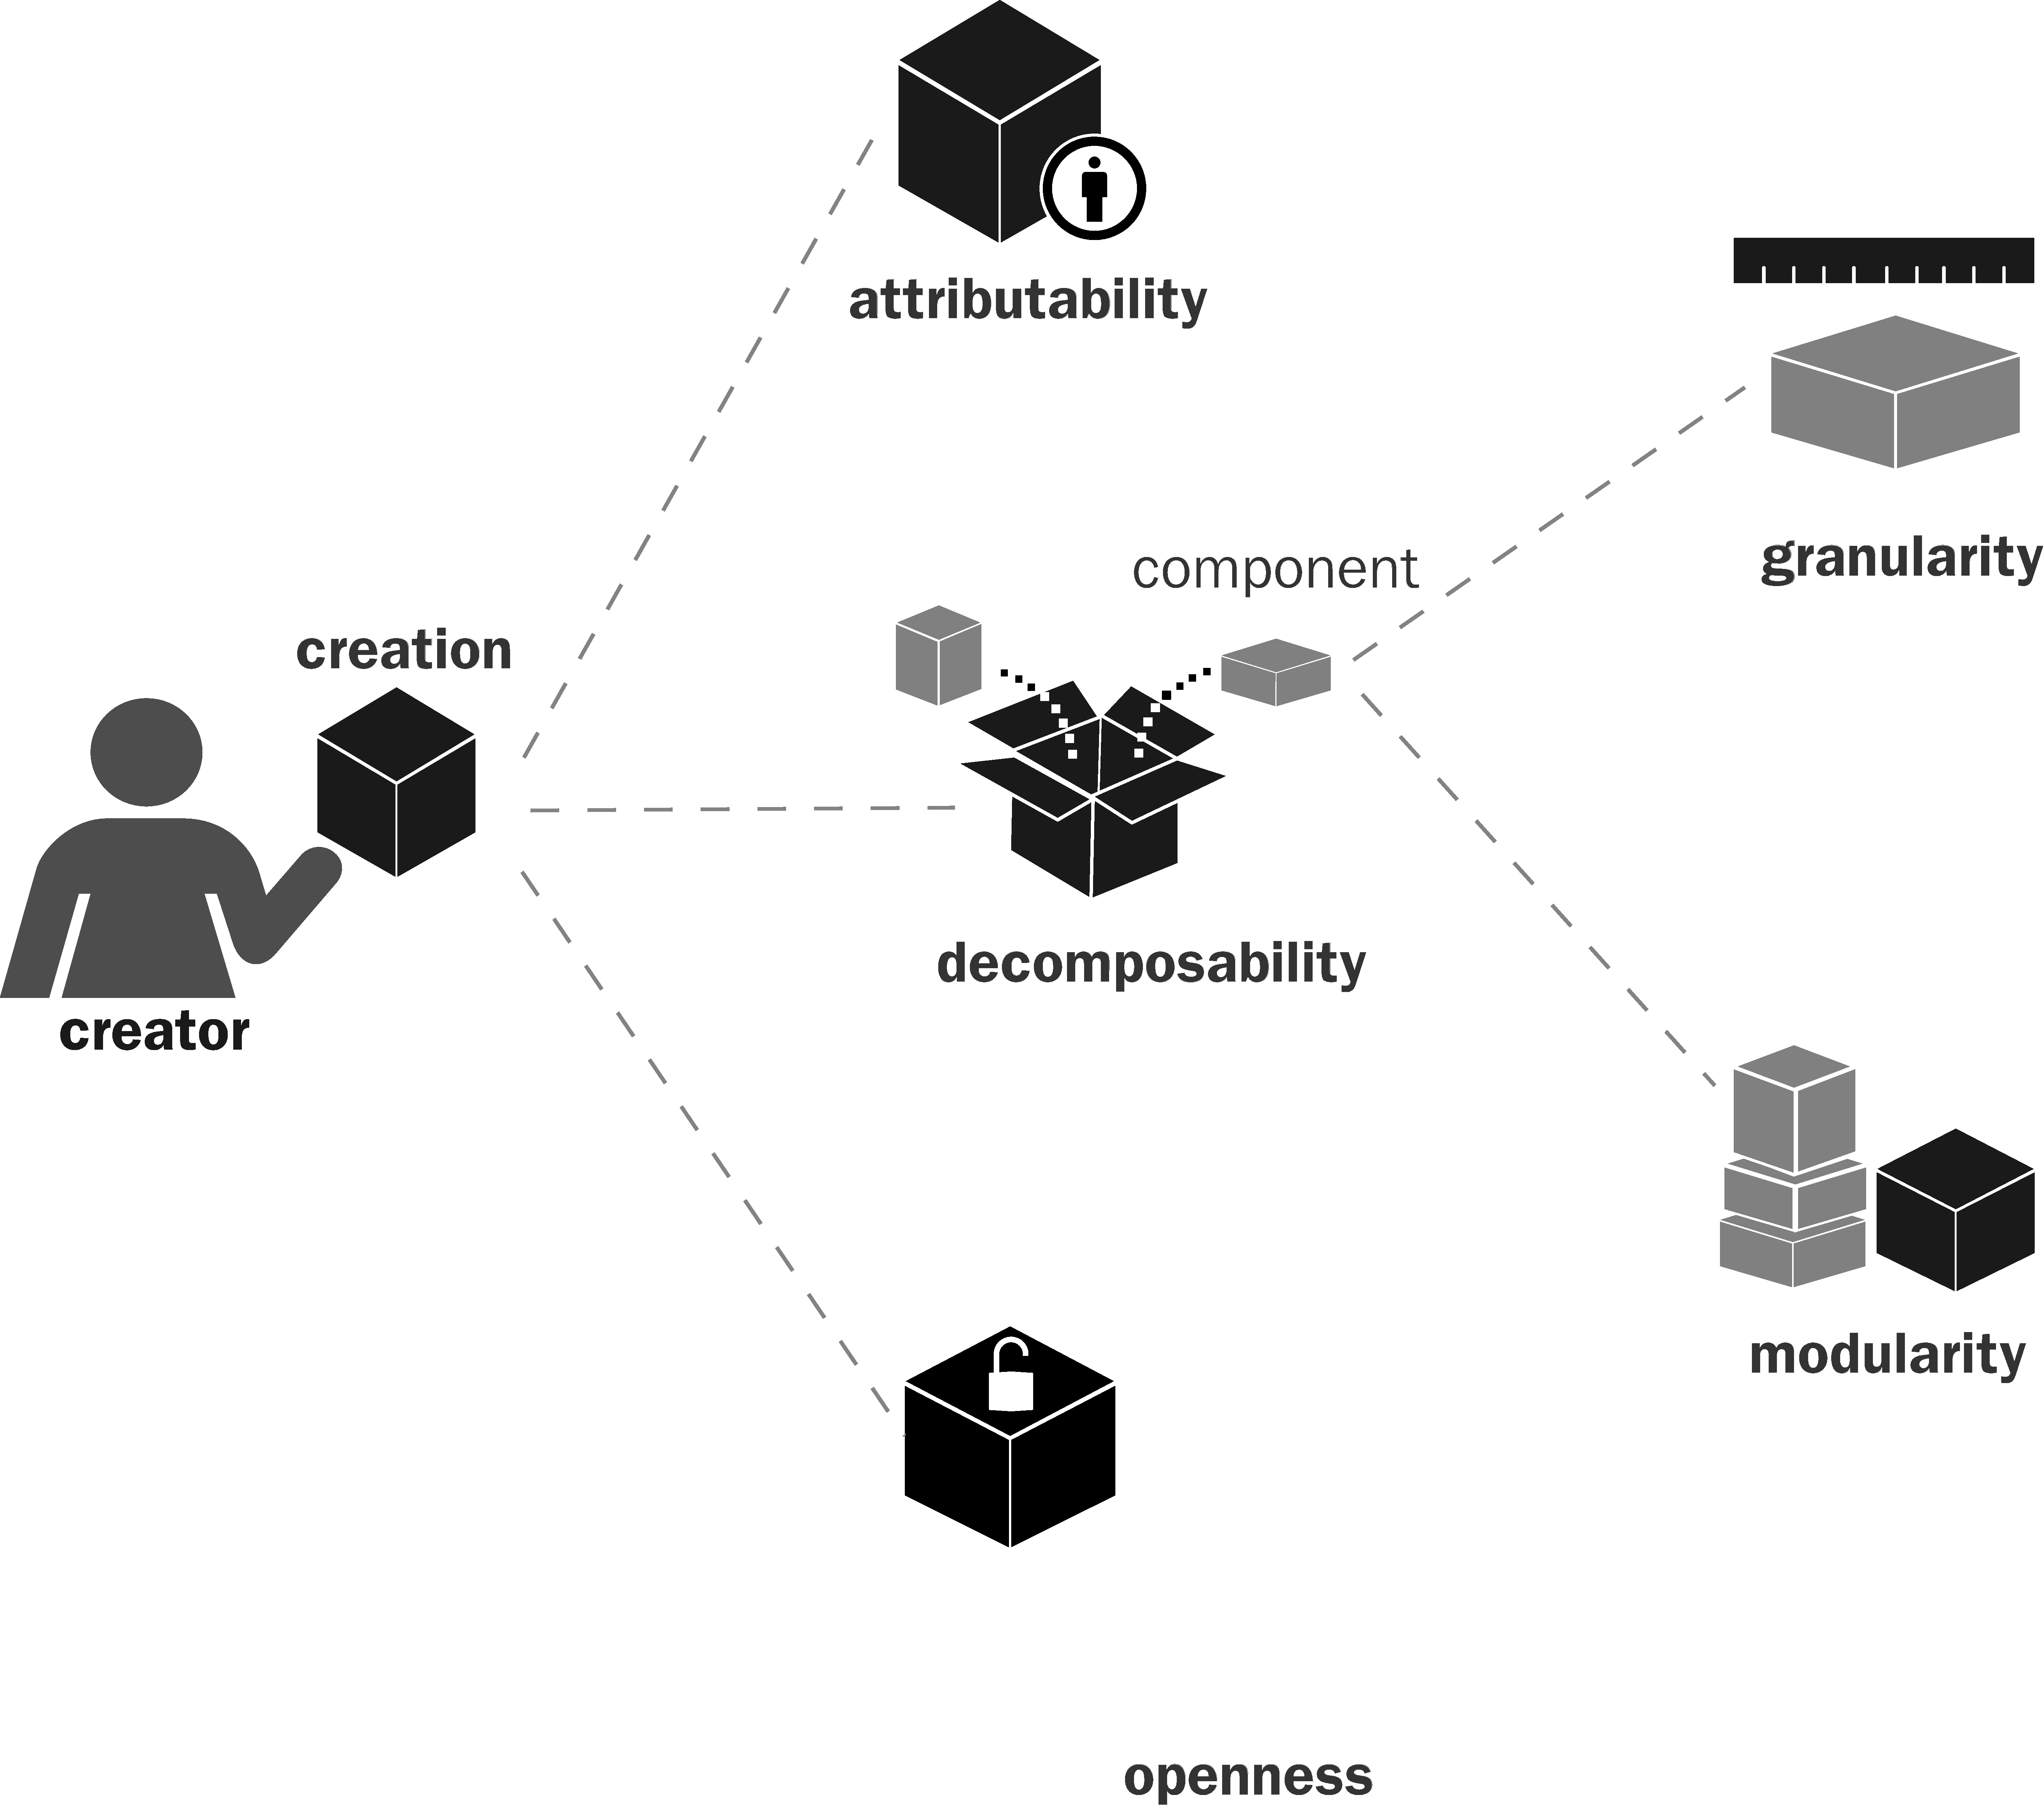
\includegraphics[width=3.25in]{figures/structure.pdf}
\caption{Structural dimensions of a remixing system}
\label{fig:structure}
\end{figure}

